\subsection{Общая информация о приложении}\label{subsec:frontcommon}
В качестве дополнительного, разивающего упражнения, с помощью инструментария Vite
разработано демонстрационное react.js-приложение, которое элегантно замыкает
разработку до ``человечного`` замкнутого решения.
В приложении доступны:
\begin{itemize}
    \item Кнопка совершения случайной покупки для демонстрации вставки в БД.
    \item Вкладка пагинированной таблицей товаров, нажатие на строки которой открывает страницу с описанием товара.
    \item Вкладка с пагинированной таблицей истории покупок.
\end{itemize}

Как отмечалось ранее, представления служат демонстрационным целям.
Также в приложении присутствует небольшое оформление, отражающее некоторые базовые правила UI/UX
касательно баланса цветов, рабочей зоны и привычных элементов интерфейса.

\begin{figure}[htbp]
    \centering
    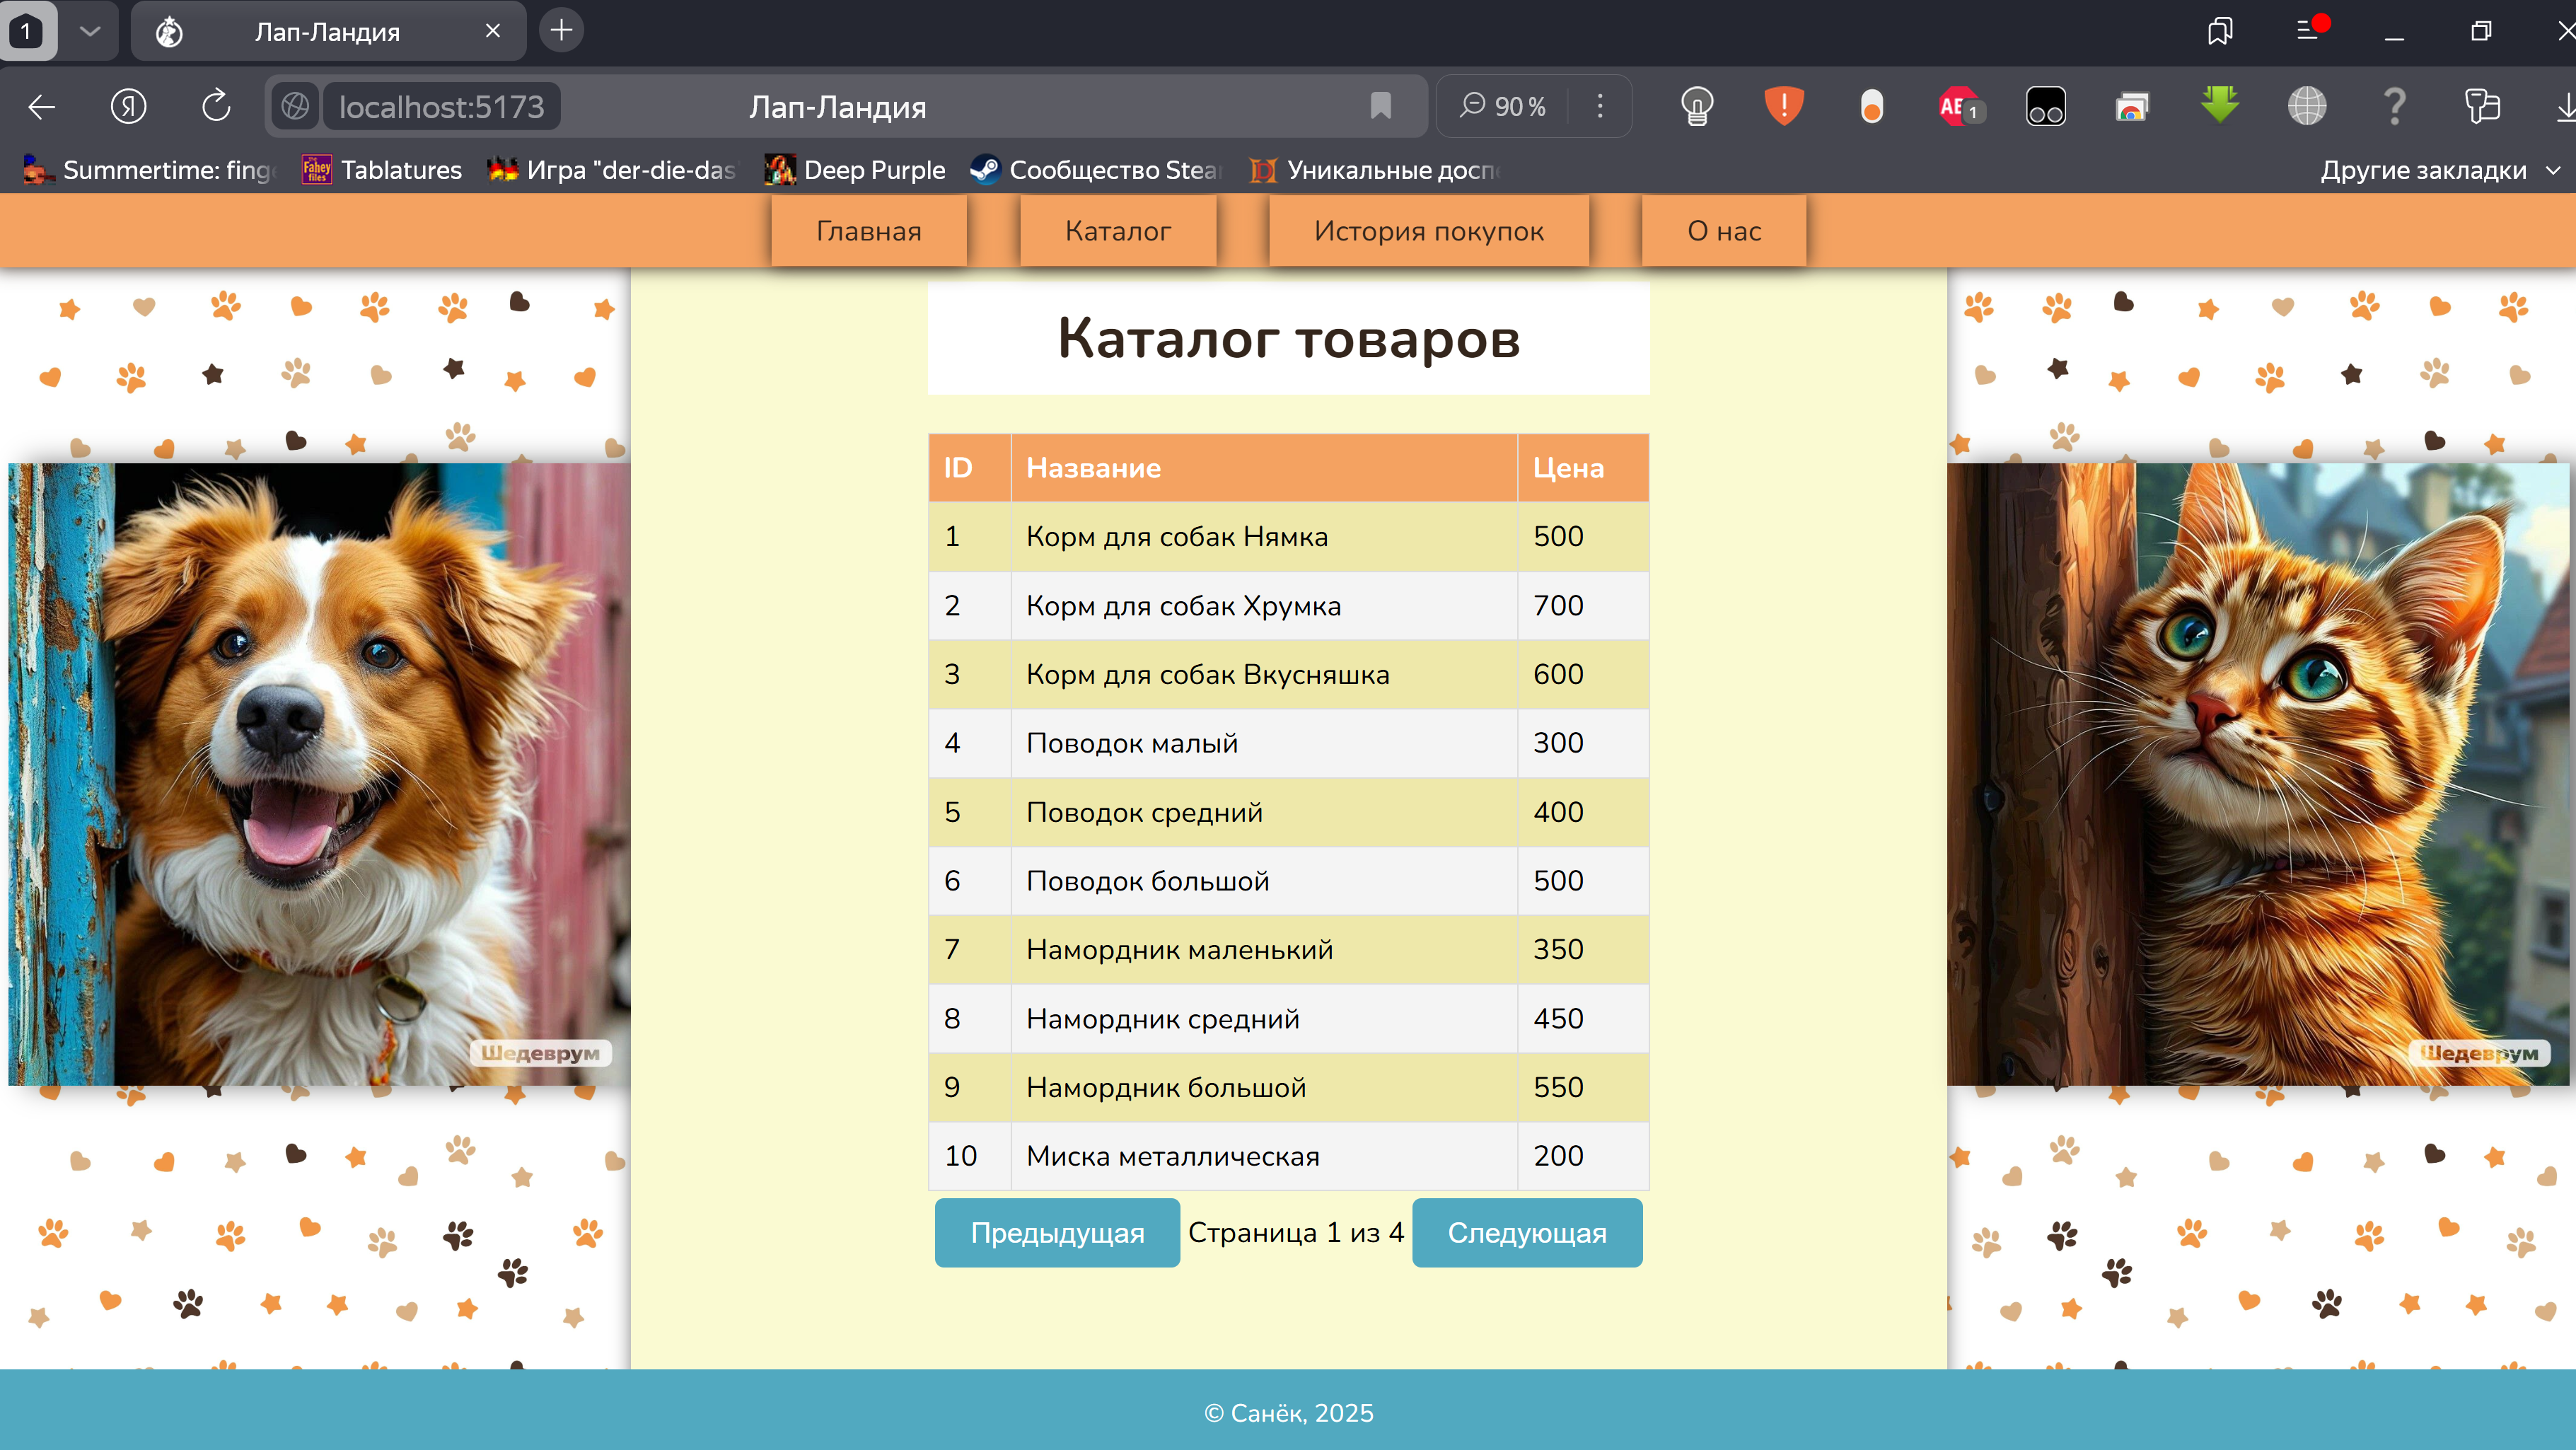
\includegraphics[width=0.9\textwidth]{browser} % Вставка изображения
    \caption{Снимок страницы клиентского приложения}\label{fig:browsershot}
\end{figure}

Изображения сгенерированы с помощью нейросети.
Иконка взята из открытых источников, со свободной лицензией.
